\documentclass{article}
\usepackage[most]{tcolorbox}
\usepackage{tikz}
\usepackage{graphicx}
\usepackage{lipsum}
\usepackage{amsfonts}
\usepackage{amsthm}
\usepackage{amssymb}
\usepackage[outputdir=../../]{minted}



\newtcolorbox{Qbox}{
enhanced,
colback=white,
}

\newcommand\questionbox[1]{%
  \begin{Qbox}#1\end{Qbox}}

\begin{document}


\subsection*{MAST90084 | Assignment 3}
Author: Sean Conlon, \texttt{sconlon@student.unimelb.edu.au} \\
Student Number: \texttt{1298865}

\vspace{10pt}
\questionbox{\textbf{Question 1.} Recall that, when expressed in the \textit{discrete hazard} function $\lambda(r, x) := P(Y = r | Y\geq r, x)$ sequential logit model has the form
$$\lambda(r, x) = \frac{\exp(\theta_r + x^T\gamma)}{1 + \exp(\theta_r + x^T\gamma)} \quad r=1,\dots,k-1$$
From this, show how you would derive the link function with components
$$\log\left\{ \frac{P(Y = r |x)}{P(Y >r|x)}\right\}=\theta_r + x^T\gamma \quad r=1,\dots,k-1$$
}
\begin{proof}
    We first note that $1 - P(Y = r | Y\geq r, x) = P(y \neq r | Y\geq r, x) = P(Y > r | x)$. It then follows from simple calculation that 
    \begin{align*}
        1 - \lambda(r, x) &= P(Y > r | x)  \\
        &= \frac{1}{1 + \exp(\theta_r + x^T\gamma)} \quad r=1,\dots,q
    \end{align*}
    it now follows 
    \begin{align*}
        \log\left\{ \frac{P(Y = r |x)}{P(Y >r|x)}\right\} &= \log P(Y = r |x) - \log P(Y >r|x) \\
        &= \log \exp(\theta_r + x^T\gamma) - \log(1+\exp(\theta_r + x^T\gamma) + \log(1+\exp(\theta_r + x^T\gamma) \\
        &=  \exp(\theta_r + x^T\gamma) \quad r =1,\dots,q
    \end{align*}
    where $q = k-1$
\end{proof}

\newpage
\questionbox{\textbf{Question 2.} The power-divergence statistic with parameter $\lambda \in \mathbb{R}$ is given by $S_\lambda=\sum_{i=1}^g \operatorname{SD}_\lambda\left(\mathbf{y}_i, \hat{\boldsymbol{\pi}}_i\right)$ where the sum of deviations over sample proportions $\mathbf{y}_i=\left(y_{i 1}, \cdots, y_{i k}\right)$ for group $i$ is
$$
\mathrm{SD}_\lambda\left(\mathbf{y}_i, \hat{\pi}_i\right)=\frac{2 n_i}{\lambda(\lambda+1)} \sum_{j=1}^k y_{i j}\left[\left(\frac{y_{i j}}{\hat{\pi}_{i j}}\right)^\lambda-1\right], \quad-\infty<\lambda<\infty .
$$

Show that substituting $\lambda=-\frac{1}{2}$, one will obtain the Freeman-Tukey statistics:
$$
S_{-\frac{1}{2}}=4 \sum_{i=1}^g \sum_{j=1}^k\left(\sqrt{n_i y_{i j}}-\sqrt{n_i \hat{\pi}_{i j}}\right)^2 .
$$
(Hint: Note that $n_i$ is the size of group $i$, and $\sum_{j=1}^k \hat{\pi}_{i j}=\sum_{j=1}^k y_{i j}=1$.)
}
\begin{proof}

\begin{align*}
    S_{-\frac{1}{2}} & =\sum_{i=1}^g \frac{2 n_i}{\left(-\frac{1}{2}\right)\left(-\frac{1}{2}+1\right)} \sum_{j=1}^k y_{i j}\left[\left(\frac{y_{i j}}{\hat{\pi}_{i j}}\right)^{-\frac{1}{2}}-1\right] \\
    & =4 \sum_{i=1}^g-2 n_i \sum_{j=1}^k y_{i j}\left[\left(\frac{\hat{\pi}_{i j}}{y_{i j}}\right)^{\frac{1}{2}}-1\right] \\
    & =4 \sum_{i=1}^g-2 n_i \sum_{j=1}^k \sqrt{y_{i j}} \sqrt{\hat{\pi}_{i j}}-y_{i j} \\
    & =4 \sum_{i=1}^g n_i\left[\sum_{j=1}^k-2 \sqrt{y_{i j}} \sqrt{\hat{\pi}_{i j}}+2 \sum_{j=1}^k y_{i j}\right] \\
    & =4 \sum_{i=1}^g n_i\left[\sum_{j=1}^k-2 \sqrt{y_{i j}} \sqrt{\hat{\pi}_{i j}}+\sum_{j=1}^k y_{i j}+\sum_{j=1}^k \hat{\pi}_{i j}\right] \\
    & =4 \sum_{i=1}^g \sum_{j=1}^k \sqrt{n_i y_{i j}}-2 \sqrt{y_{i j}} \sqrt{\hat{\pi}_{i j}}+\sqrt{n_i \hat{\pi}_{i j}} \\
    & =4 \sum_{i=1}^g \sum_{j=1}^k\left(\sqrt{n_i y_{i j}}-\sqrt{n_i \hat{\pi}_{i j}}\right)^2
\end{align*}
\end{proof}


\newpage
\questionbox{\textbf{Question 3.} }


\newpage
\questionbox{\textbf{Question 4.}  You need to install the \texttt{R} packages \texttt{gee} and \texttt{MASS} for doing this question. The question focuses on analysing the OME data stored in MASS. Type \texttt{help(OME)} and \texttt{help(gee)} to get details of the data and GEE solver.}

\questionbox{\textbf{a)} How many children were included in the data}

Calling \texttt{?OME} in the R Console brings up the corresponding documentation for the data set. Within the description for subject \texttt{ID} it reads \textit{Subject ID (1 to 99, with some IDs missing). A few subjects were measured at different ages.} From this, we infer the data set contains 99 children.

\questionbox{\textbf{b)}  How many tests did the child with ID=1 attend to in the data? (Namely, what is the cluster size associated with child 1?) }
\begin{minted}{R}
    data <- OME
    nrow(data[data$ID == 1, ])
\end{minted}
Shows the cluster size for \texttt{ID = 1} is 20.

\questionbox{\textbf{d)}  Give the commands for finding the estimates and their robust variance matrix for the regression parameters in the marginal model. DO NOT use the \texttt{summary()} function. Please also show the numbers.}
\begin{minted}{R}
     fm <- gee(cbind(Correct, Trials - Correct) ~ Loud + Age + OME + Noise, id = ID,
             data = OME, family = binomial, corstr = "exchangeable", scale.fix = F)

    fm$coefficients
    fm$robust.variance
\end{minted}
The bottom two lines produce the regression coefficients and robust variance matrix respectively. Their outputs are as follows; for the coefficients:
\begin{center}
    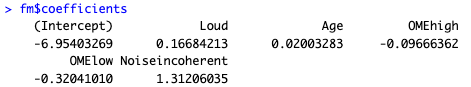
\includegraphics[scale=0.5]{glm-notes/Assignments/assignment-imgs/coefs.png}
\end{center}
and for the robust variance:
\begin{center}
    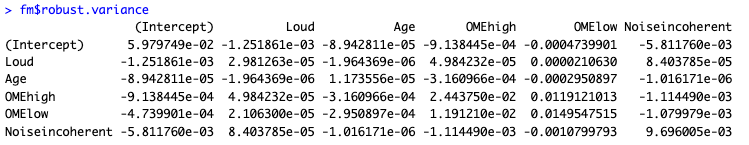
\includegraphics[scale=0.5]{glm-notes/Assignments/assignment-imgs/robustvar.png}
\end{center}

\end{document}

%family=negative_binomial(1/theta, link=log)
%beta_new = abovefit\$coef